\chapter{Case study of influenza A H1N1}
\label{influenza}

\section{Abstract}

This is an ongoing collaborative project with Prof. Pang-Chui Shaw and Edwin Lo from School of Biomedical Sciences, Chinese University of Hong Kong, Hong Kong.

\section{Background}

According to the fact sheets of World Health Organization, available at http://www.who.int/mediacentre/factsheets/fs211/en/, influenza viruses has been causing sporadic pandemics and annual epidemics worldwide, claiming 250,000 to 500,000 lives and resulting in about 3 to 5 million cases of severe illness each year. The H5N1 bird flu outbreak in Hong Kong in 1997, the H1N1 swine flu outbreak in Mexico in 2009, and the ever-present threat of H5N1 acquiring human-to-human transmission capability remind us of the imminent danger posed by the influenza viruses. 

Influenza viruses are negative-sense single-stranded RNA viruses. They are classified into types A, B and C based on the antigenic difference in their nucleoproteins and matrix proteins. Influenza A is the major pathogen for most cases of epidemic influenza. The influenza A genome comprises 8 segments of RNA coding for 11 proteins, which are hemagglutinin (HA), neuraminidase (NA), matrix protein 1 (M1), M2 proton channel, nucleoprotein (NP), non-structural protein 1 (NS1), nuclear export protein (NEP), polymerase acid protein (PA), polymerase basic proteins (PB1 and PB2) and PB1-F2. Influenza A viruses are further organized into 16 hemagglutinin subtypes (H1-H16) and 9 neuraminidase subtypes (N1-N9) according to their distinct antigenic properties.

To date, four antiviral drugs have been approved by the US FDA (Food and Drug Administration). They are two NA inhibitors, oseltamivir (Tamiflu\textsuperscript{\textregistered}) and zanamivir (Relenza\textsuperscript{\textregistered}), and two M2 channel blockers, amantadine (Symmetrel\textsuperscript{\textregistered}) and rimantadine (Flumadine\textsuperscript{\textregistered}). Unfortunately, three of them, oseltamivir, amantadine, rimantadine, are now found to be ineffective against circulating strains due to the rapid emergence of drug-resistant viral mutations in pandemic and seasonal influenza viruses. Besides, amantadine and rimantadine exhibit side effects on the central nervous system. These alarming facts highlight the urgent need for designing new anti-influenza drugs.

The life cycle of influenza viruses has been well studied \citep{1539,1522,1559} and nearly all the viral proteins have become potential therapeutic targets \citep{1539,1229,1519}. Oseltamivir and zanamivir target the active site of NA. Amantadine and rimantadine target the inside pore near Ser31 of M2. Neu5Ac (N-acetylneuraminic acid) targets the sialic acid binding site of HA. TBHQ (tert-butylhydroquinone) targets the TBHQ binding site of HA. No inhibitors have been firmly established for the other 8 viral proteins, but leads have been proposed in some cases.

In this study we concentrate on discovering inhibitors of three viral proteins: NP, PA and PB2. These proteins are structurally related in that NP forms homo-oligomers and multiple copies of NP wrap around genomic RNA, along with a trimeric polymerase of subunits PA, PB1 and PB2 making up a ribonucleoprotein (RNP) complex.

\subsection{Nucleoprotein (NP)}

NP is a polypeptide of 498 amino acids, and folds into a crescent shape with a head and a body domain. Functionally speaking, NP not only encapsidates the viral RNA, but also forms homo-oligomers. NP homo-oligomerizes by inserting the tail loop (amino acids 402 to 428) into the groove of the body domain of its neighboring NP molecule.

The tail loop makes extensive interactions with the binding groove through intermolecular $\beta$-sheets, hydrophobic interactions and salt bridges \citep{1140}. The amino acids in the tail-loop binding groove for nucleoprotein oligomerization are identical among several influenza A strains, and the displacement of the tail loop from its binding pocket causes significant structural rearrangements in nucleoprotein and completely abolishes the replication and transcription functions \citep{1231}.

Chemical compounds which competitively displace the tail loop from its binding pocket would interfere with viral genome replication, and therefore serve as promising compounds for anti-influenza drug development \citep{1140,1231,1232}. The tail-loop peptide can inhibit nucleoprotein oligomerization and slow down viral replication. A potent inhibitor of nucleoprotein of wild-type and mutant strains has been identified through virtual screening \citep{1233}.

So far, two crystal structures of influenza A NP have been solved, they are from the H1N1 strain (PDB code: 2IQH) \citep{1140} and the H5N1 strain (PDB code: 2Q06) \citep{1231}. \citep{1140} used X-ray crystallography and reported a 3.2\AA resolution structure of a homologous NP from human origin (A/WSN/1933; H1N1) (PDB: 2IQH). \citep{1231} 3.3\AA crystal structure of A/HK/483/97 (H5N1) NP (PDB: 2Q06) from avian origin. H5N1 NP and H1N1 NP share 94\% sequence identity, and after aligning 398 residues (residues 22–72, 92–202, 213–396, 438–489) the root mean square deviation (RMSD) between the two crystal structures is 1.0\AA \citep{1140}. The interaction of the tail loop of one NP molecule with the neighboring protomer in H5N1 and H1N1 is virtually identical \citep{1140}.

Multiple sequence alignment of more than 2500 influenza A NP showed that NP is highly conserved, and for NP tail loops the tertiary structure conservation is correlated to the conserved primary sequence \citep{1517}. Therfore NPs an attractive candidate for inhibitor design. The high degree of conservation in sequence identity and structure makes NP an ideal target for the development of broad spectrum influenza drug.%\citep{1561} Mutational Analysis of Conserved Amino Acids in the Influenza A Virus Nucleoprotein

\citep{1447} used cryo-electron microscopy and determined the 3D structure of a biologically active recombinant RNP that reveals the NP-NP interaction domain. Mutants R416A and F412A were strongly affected in replication, whereas mutants S413T, F420A, K422A and S423A behaved as wild type. The contacts of amino acid R416 and F412 are essential for replication, while amino acid K422 does not appear to be important, in spite of being conserved among type A and B viruses.

\citep{1232} used an RNP reconstitution assay and identified eight NP single- or double-point mutants that had different degrees of defects in forming functional RNPs. These mutants were I406S, V408S P410S, R416A, L418S P419S and R422A at the tail loop, and R267A, E339A and E449A at the insertion groove, with charged residues mutated to alanine to remove the hydrogen bond interaction while other residues mutated to serine to remove the hydrophobic interaction. Among the three mutants at the insertion groove, the E339A mutant totally abolished the RNP activities, and the R267A and E449A mutants decreased the RNP activities by more than 50\%. In contrast, the T390S mutant did not show a significant change in the RNP activities. Further characterization showed that the E339A mutant existed as monomers \textit{in vitro}, and also \textit{in vivo} in the absence of RNA, deviating from the trimeric or oligomeric form of wild-type NP. Although the R267A mutant retained 45\% of the RNP activity, surprisingly it appeared as a monomer \textit{in vitro}. It resumed an oligomeric form upon the addition of RNA and retained a certain degree of RNP activity \textit{in vivo}. The E449A mutant existed as a mixture of unstable oligomers, and the R422-E449 ion pair stabilized the NP homo-oligomer. These results may indicate that E339 is essential while R267 and E449 are important for the NP homo-oligomerization process.

\citep{906} used a forward chemical genetics approach and identified NP as a druggable target and found a lead compound, nucleozin, with efficacy \textit{in vitro} and in animal studies, that triggers NP aggregation and thereby inhibits its nuclear accumulation, leading to cessation of viral replication. \citep{1515} developed a screening procedure to search for antiinfluenza inhibitors from 1.2 million compounds, and established a high throughout virus yield reduction methodology to confirm hits. It identified previously reported antiinfluenza compounds as well as new ones. Several antiinfluenza compounds, including nucleozin and its analogs, were inhibitory to the influenza RNA-dependent RNA polymerase (RdRP). \citep{1233} reported a rational approach to target influenza virus with a new mechanism of NP-NP interaction disruption. E339A and R416A were unable to support viral replication in the absence of wild type NP, demonstrating the importance of the salt bridge between E339 lining the binding pocket and R416 on the tail loop in viral survival and establishing the salt bridge as a sensitive antiinfluenza target. Peptides encompassing R416 were shown to disrupt NP-NP interaction and inhibit viral replication. Virtual screening of 1,775,422 compounds was performed to target E339...R416 and some small molecules identified were shown to disrupt the formation of NP trimers and inhibit replication of wild type and nucleozin-resistant strains. \citep{1516} utilized nucleozin as a lead molecule and designed and synthesized a series of 1\textit{H}-1,2,3-triazole-4-carboxamide derivatives as new anti-influenza A agents targeting influenza virus nucleoproteins.

\citep{1520} A Novel Small Molecule Inhibitor of Influenza A Viruses that Targets Polymerase Function and Indirectly Induces Interferon.%26 Apr 2012
\citep{1519} Antivirals Targeting Influenza A Virus.%21 May 2012
\citep{1521} Nucleozin Targets Cytoplasmic Trafficking of Viral Ribonucleoprotein-Rab11 Complexes in Influenza A Virus Infection.%Apr 2013
\citep{1522} A comprehensive map of the influenza A virus replication cycle.%2 Oct 2013
\citep{1524} A small molecule multi-kinase inhibitor reduces influenza A virus replication by restricting viral RNA synthesis.%Oct 2013
\citep{1550} Structural Investigation of Cycloheptathiophene-3-carboxamide Derivatives Targeting Influenza Virus Polymerase Assembly.%Dec 2013
\citep{1513} Large-scale analysis of influenza A virus nucleoprotein sequence conservation reveals potential drug-target sites.%22 Feb 2014
\citep{1527} Optimization of Small-Molecule Inhibitors of Influenza Virus Polymerase: From Thiophene-3-Carboxamide to Polyamido Scaffolds.%May 2014
\citep{1526} Screening and identification of inhibitors against influenza A virus from a US drug collection of 1280 drugs.%24 Jun 2014
\citep{1523} Emerging antiviral resistant strains of influenza A and the potential therapeutic targets within the viral ribonucleoprotein (vRNP) complex.%16 Sep 2014
\citep{1525} Antiviral strategies against influenza virus: towards new therapeutic approaches.%Oct 2014
\citep{1549} Emerging antiviral resistant strains of influenza A and the potential therapeutic targets within the viral ribonucleoprotein (vRNP) complex.

\begin{figure}
\centering
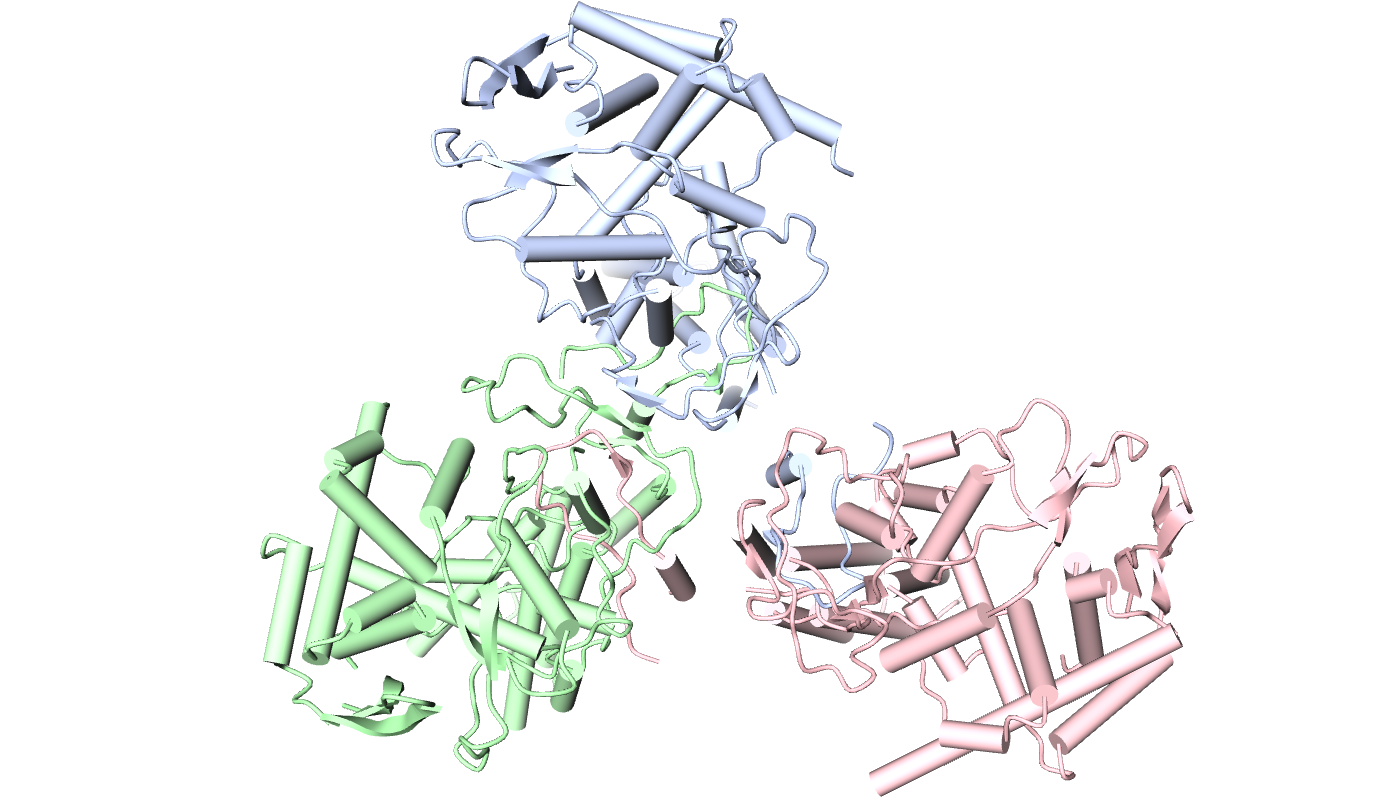
\includegraphics[width=\linewidth]{../influenza/2IQH.png}
\caption{Nucleoprotein trimer with three subunits shown in different colors. The flexible tail loop of a nucleoprotein molecule is inserted into the body domain of an adjacent nucleoprotein molecule.}
\label{influenza:2IQH}
\end{figure}

\subsection{Polymerase acidic protein (PA)}

%\citep{1540} Crystal structure of the polymerase PAC–PB1N complex from an avian influenza H5N1 virus.%Aug 2008
%\citep{1547} Detection and Characterization of Influenza A Virus PA-PB2 Interaction through a Bimolecular Fluorescence Complementation Assay.%Apr 2009
%\citep{1541} Identification of High-Affinity PB1-Derived Peptides with Enhanced Affinity to the PA Protein of Influenza A Virus Polymerase.%Feb 2011
%\citep{1545} Screening Anti-influenza Agents that Target Avian Influenza Polymerase Protein PAC from Plant Extracts Based on NMR Methods.%Jun 2011
%\citep{1543} NMR identification of anti-influenza lead compound targeting at PAC subunit of H5N1 polymerase.%early 2012
%\citep{1548} Screen Anti-influenza Lead Compounds That Target the PAC Subunit of H5N1 Viral RNA Polymerase}.%Aug 2012
%\citep{1542} High-throughput docking for the identification of new influenza A virus polymerase inhibitors targeting the PA–PB1 protein–protein interaction.%Jan 2014
%\citep{1544} Involvement of the N-terminal portion of influenza virus RNA polymerase subunit PB1 in nucleotide recognition.%early 2014

The influenza A RNA polymerase is a heterotrimer composed of three subunits, namely PA, PB1 and PB2. It binds the conserved 3' and 5' ends of each of the 8 single-stranded RNA segments in the influenza A virus genome. All the three subunits are required for both transcription and replication. PA is involved in assembly of the functional complex, cap binding and vRNA (virion RNA) promoter binding. PB1 carries the polymerase active site. PB2 includes the capped-RNA recognition domain.

The carboxy-terminal domain of PA forms a deep and highly hydrophobic groove (residues 257-716) into which the amino-terminal residues of PB1 (residues 1-16) can fit by forming a helix and interact through an array of hydrogen bonds and hydrophobic contacts \citep{1141} (Figure \ref{influenza:2ZNL}). The loss of PA abolishes RNA polymerase activity and viral replication. PA and its interface with PB1 are therefore potential drug targets \citep{1141}. A peptide corresponding to the N-terminal 25 residues of PB1 inhibits the polymerase activity and viral replication, presumably by blocking the assembly of the polymerase trimer \citep{1234}. A novel inhibitor targeting the PA-PB1 binding site has been discovered by virtual screening \citep{1235}.

\subsection{Polymerase basic protein 2 (PB2)}

%\citep{1552} The RNA Polymerase PB2 Subunit of Influenza A HongKong 156 1997 (H5N1) Restrict the Replication of Reassortant Ribonucleoprotein Complexes.%Feb 2012
%\citep{1553} Computational Studies on the Substrate Interactions of Influenza A Virus PB2 Subunit.%Sep 2012
%\citep{1551} Crystallization and X-ray crystallographic analysis of the cap-binding domain of influenza A virus H1N1 polymerase subunit PB2.%Jan 2013
%\citep{1554} Structural and Functional Characterization of K339T Substitution Identified in the PB2 Subunit Cap-binding Pocket of Influenza A Virus.%Feb 2013
%\citep{1557} New 7-Methylguanine Derivatives Targeting the Influenza Polymerase PB2 Cap-Binding Domain.%Oct 2013
%\citep{1546} Conformational Polymorphism of m7GTP in Crystal Structure of the PB2 Middle Domain from Human Influenza A Virus. Coordinates and structure factors of PB2 middle domain with two amino acids mutation (P453H and I471T) have been deposited in the Protein Data Bank. The accession numbers of the structure without m7GTP and with m7GTP are 3WI0 and 3WI1, respectively. Additionally, wild type of PB2 middle domain without m7GTP has been deposited with the accession number 4J2R.%Nov 2013
%\citep{1560} Comparative Structural and Functional Analysis of Orthomyxovirus Polymerase Cap-Snatching Domains.%Jan 2014
%\citep{1555} Crystallization and preliminary X-ray diffraction studies of a surface mutant of the middle domain of PB2 from human influenza A (H1N1) virus.%early 2014
%\citep{1558} Discovery of a Novel, First-in-Class, Orally Bioavailable Azaindole Inhibitor (VX-787) of Influenza PB2.%Jul 2014
%\citep{1556} Novel residues in avian influenza virus PB2 protein affect virulence in mammalian hosts.%Oct 2014

PB2 binds the 5' cap of host pre-mRNAs, which are cleaved after 10-13 nucleotides by the endonucleolytic activity of PB1. Residues 318-483 of PB2 form the cap-binding domain (Figure \ref{influenza:2VQZ}). An inhibitor of cap-snatching activities of PB2 has been identified by high-throughput screening \citep{1236}.

\begin{figure}
\centering
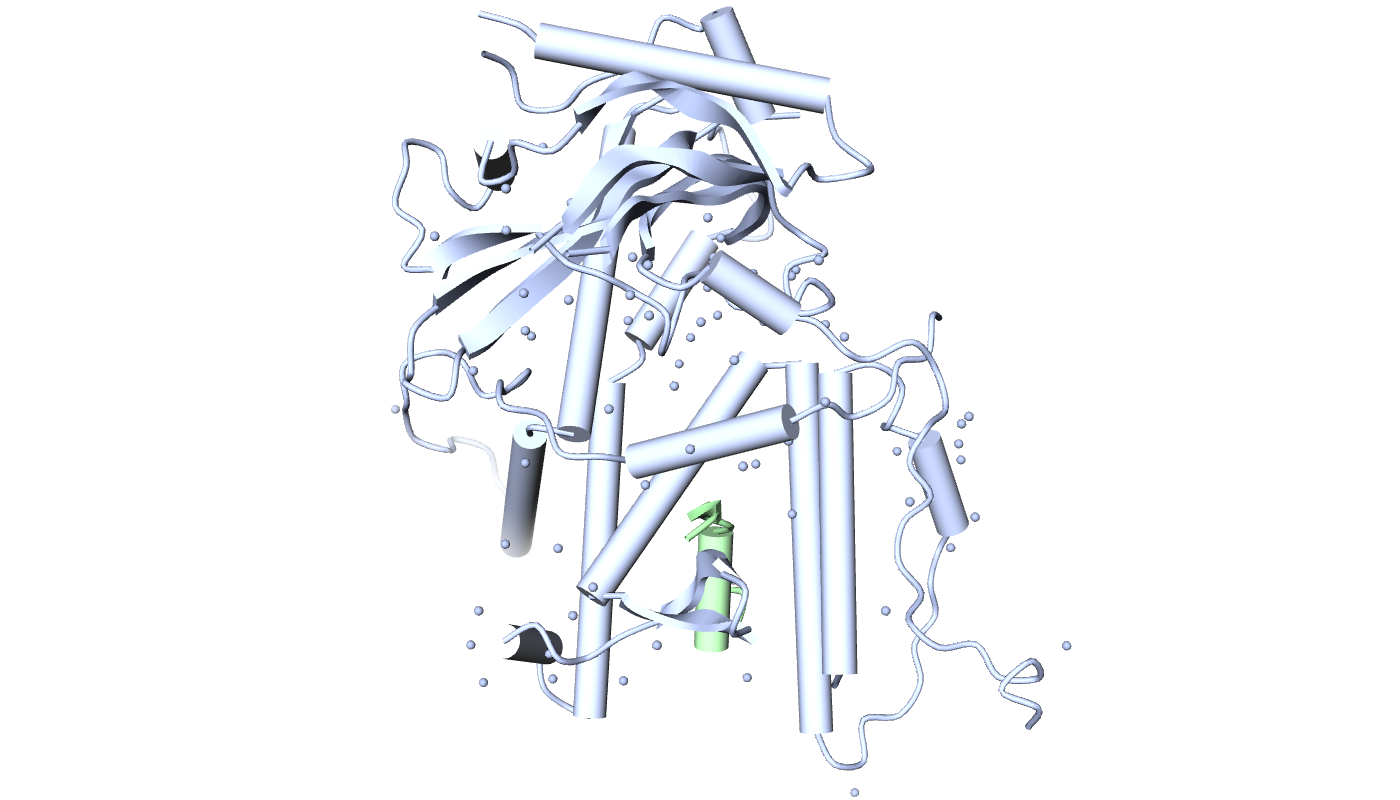
\includegraphics[width=\linewidth]{../influenza/2ZNL.png}
\caption{Crystal structure of the C-terminal domain of PA, colored in green, bound to the N-terminal peptide of PB1, colored in orange.}
\label{influenza:2ZNL}
\end{figure}

\begin{figure}
\centering
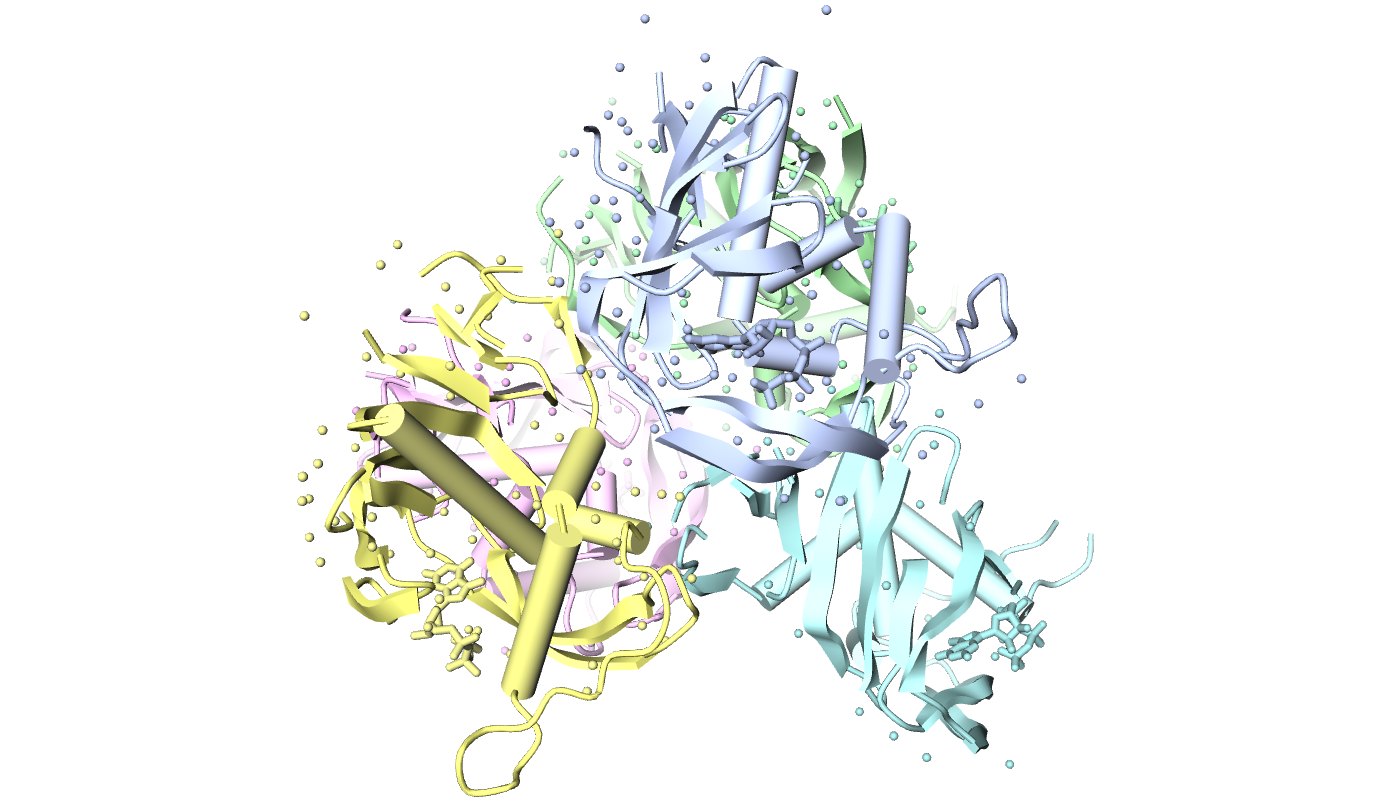
\includegraphics[width=\linewidth]{../influenza/2VQZ.png}
\caption{PB2 cap binding domain (amino acids 318 to 483) in complex with m\textsuperscript{7}GTP.}
\label{influenza:2VQZ}
\end{figure}

\section{Motivation}



\section{Objective}

We used the approach of structure-based virtual screening to discover promising ligands against the nucleoprotein (NP), the polymerase acidic protein (PA) and the polymerase basic protein 2 (PB2). Specifically, this virtual screening campaign was done by idock \citep{1153}.

\section{Methods}

We employed structure-based virtual screening on nucleoprotein and polymerase subunits PA and PB2 in order to identify novel class of anti-influenza drugs. We obtained the X-ray crystal structures of influenza viral nucleoprotein with PDB ID 2IQH \citep{1140}, influenza A RNA polymerase subunits PA-PB1 complex with PDB ID 2ZNL \citep{1141}, and subunit PB2 in complex with m\textsuperscript{7}GTP with PDB ID 2VQZ \citep{1192}. For the nucleoprotein, we removed chains B and C and only retained chain A. For the PA-PB1 complex, we removed PB1 and only retained PA. For the PB2-m\textsuperscript{7}GTP complex, we removed PB2 chains B, D, E, F and m\textsuperscript{7}GTP and only retained PB2 chain A. Using idock 1.5 with a fine grid map granularity of 0.08\AA, we docked 7,220,835 ZINC \citep{532} clean ligands against nucleoprotein chain A and 73,648 ZINC clean ligands against PA. All the ligands are free of yuck compounds and have a molecular weight of at least 350g/mol. The docking took us 5 months. Later on we developed idock 1.6 and used it to dock 1,869,678 ligands against PB2 with vendor information available.

\section{Results}

Figures \ref{influenza:2IQH-ZINC20464531} and \ref{influenza:2IQH-ZINC33733935} depict the interactions between influenza viral nucleoprotein chain A and two high-rank ligands. Figures \ref{influenza:2ZNL-ZINC17206951} and \ref{influenza:2ZNL-ZINC40879809} depict the interactions between influenza A RNA polymerase subunit PA and two high-rank ligands. Figures \ref{influenza:2VQZ-ZINC03015113} and \ref{influenza:2VQZ-ZINC08386295} depict the interactions between influenza A RNA polymerase subunit PB2 and two high-rank ligands.

\begin{figure}
\centering
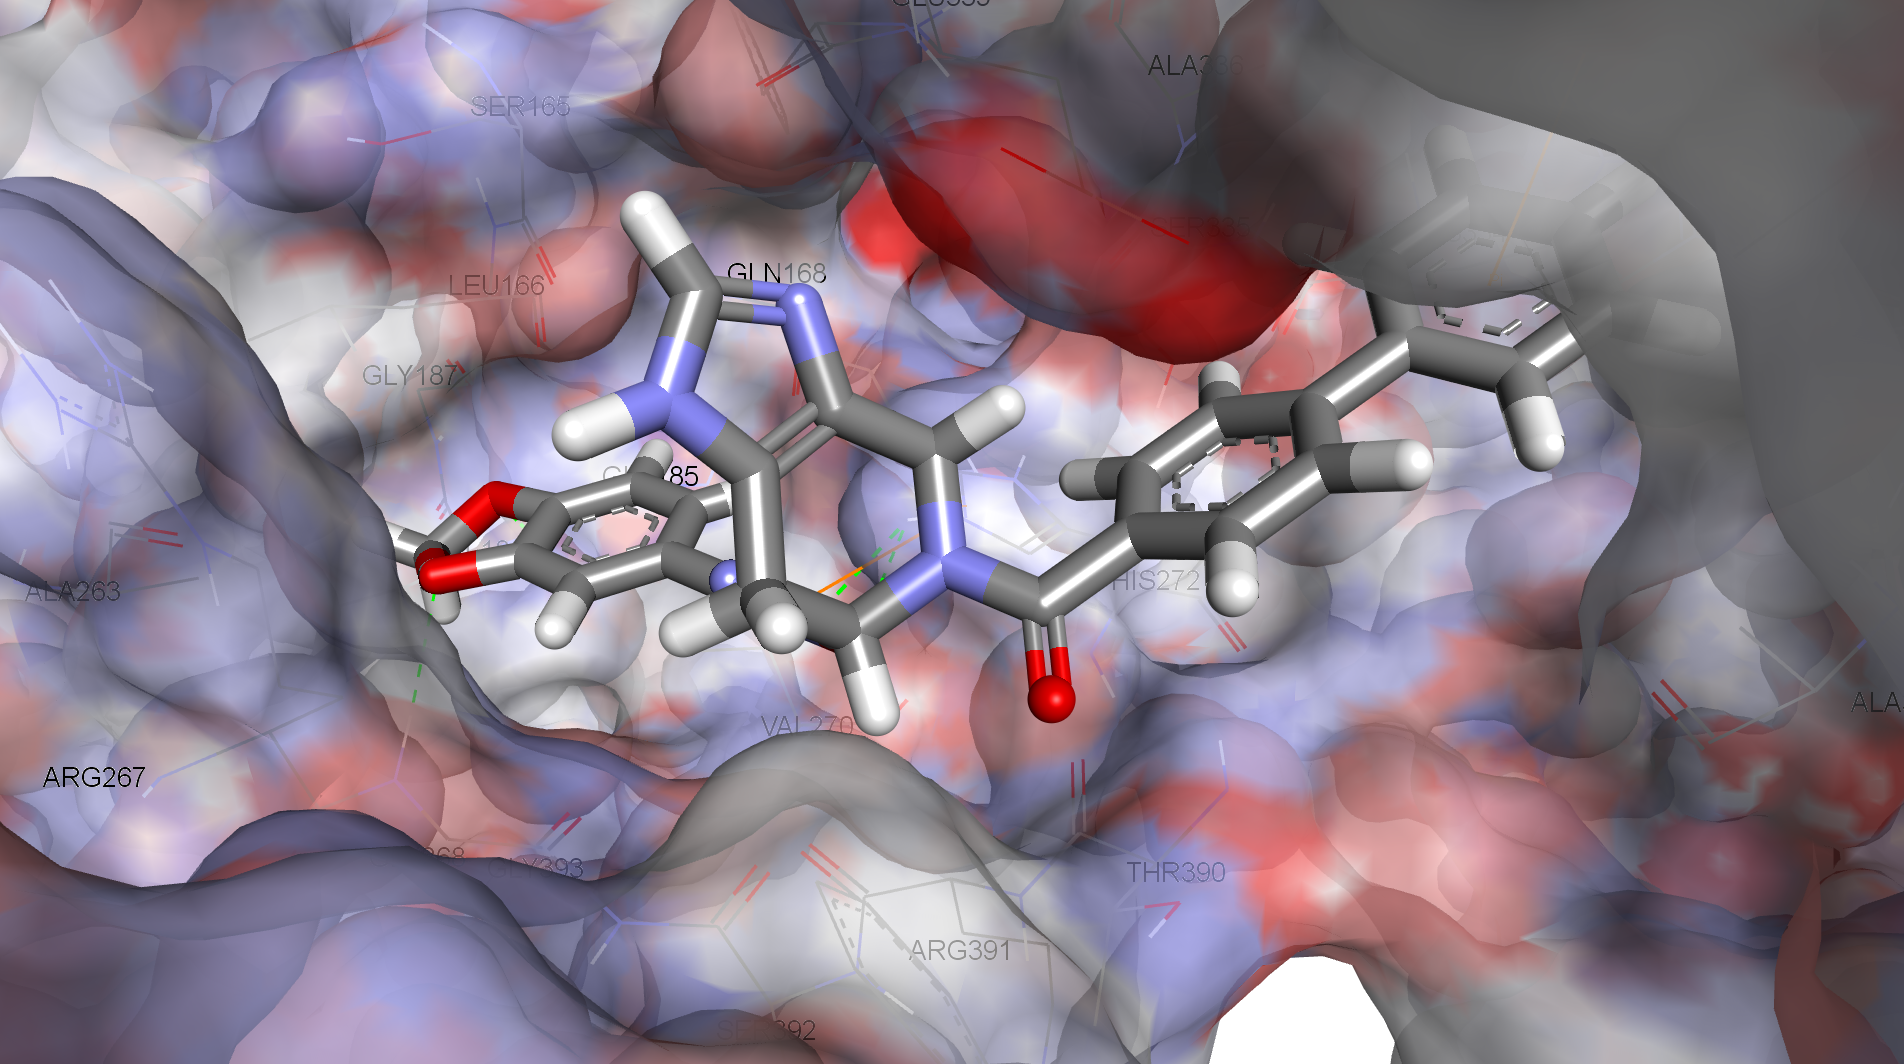
\includegraphics[width=\linewidth]{../influenza/2IQH-ZINC20464531.png}
\caption{Influenza viral nucleoprotein chain A in complex of ZINC20464531, which forms 4 hydrogen bonds with VAL186, GLY268 and HIS272, Pi-Pi interactions with TRP330, and Pi-Cation interaction with HIS272 and ARG389. Free energy predicted by idock is -13.305 kcal/mol.}
\label{influenza:2IQH-ZINC20464531}
\end{figure}

\begin{figure}
\centering
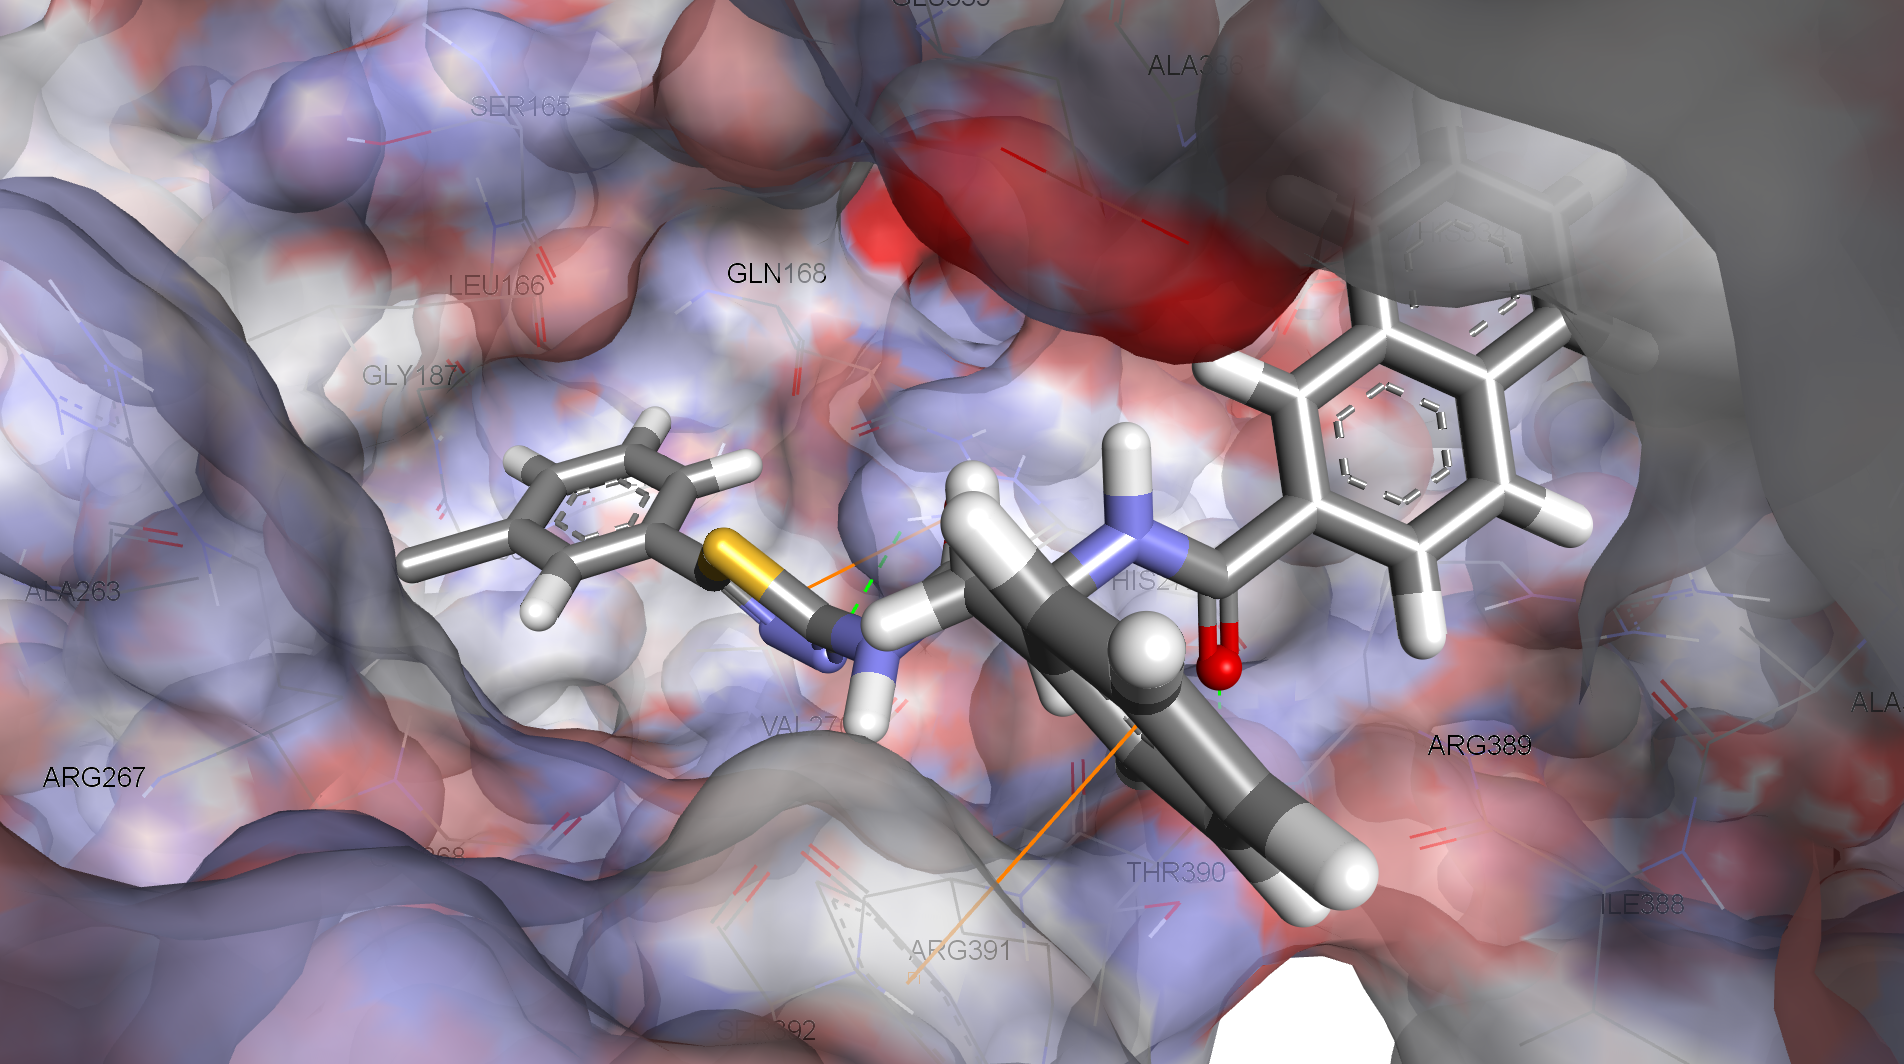
\includegraphics[width=\linewidth]{../influenza/2IQH-ZINC33733935.png}
\caption{Influenza viral nucleoprotein chain A in complex with ZINC33733935, which forms 2 hydrogen bonds with HIS272 and THR390, Pi-Pi interactions with PHE458, and Pi-Cation interaction with HIS272. Free energy predicted by idock is -13.220 kcal/mol.}
\label{influenza:2IQH-ZINC33733935}
\end{figure}

R267
G268
H272
A337
F338
E339
D340
R342
A387
I388
T390
E449
P453
S457
N459
G460
R461
I475
S478
F488

\begin{figure}
\centering
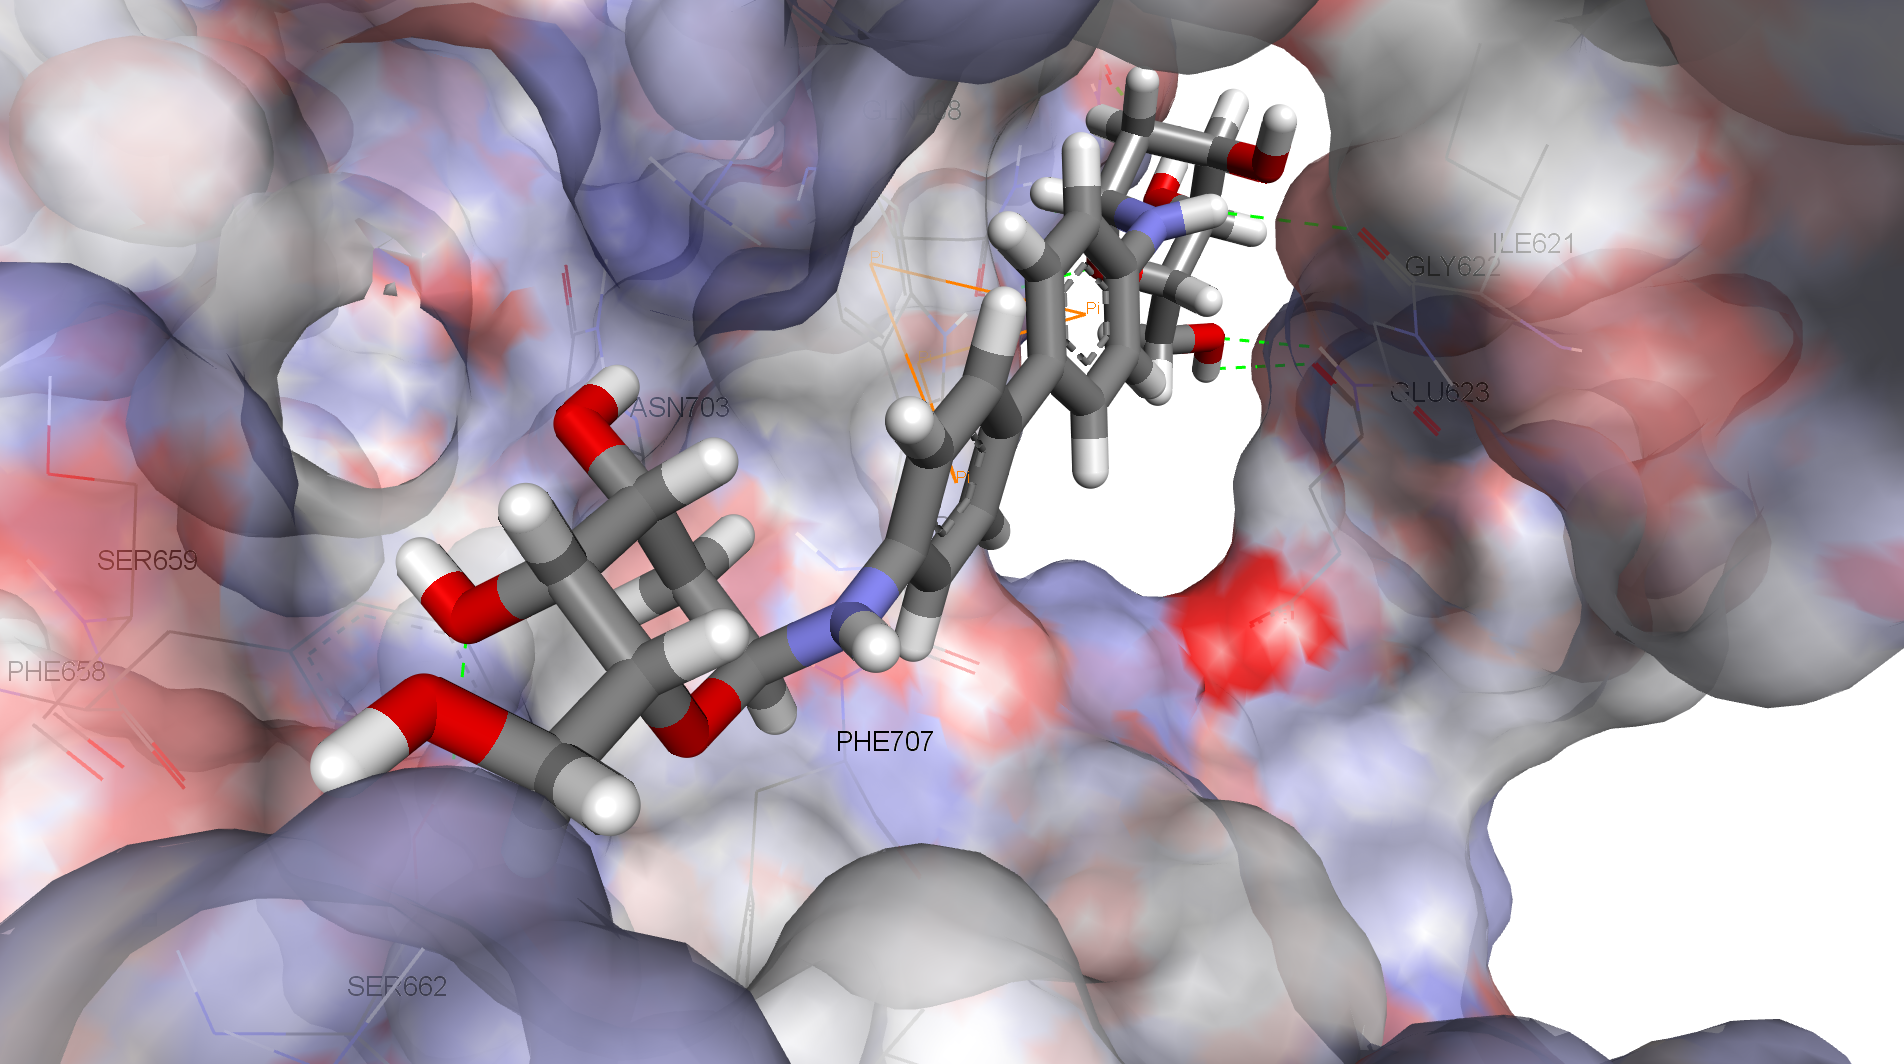
\includegraphics[width=\linewidth]{../influenza/2ZNL-ZINC17206951.png}
\caption{Influenza A RNA polymerase subunit PA in complex of ZINC17206951, which forms 8 hydrogen bonds with GLN408, ASN412, ILE621, GLU623, SER662 and ASN703, and Pi-Pi interactions with TRP706. Free energy predicted by idock is -9.562 kcal/mol.}
\label{influenza:2ZNL-ZINC17206951}
\end{figure}

\begin{figure}
\centering
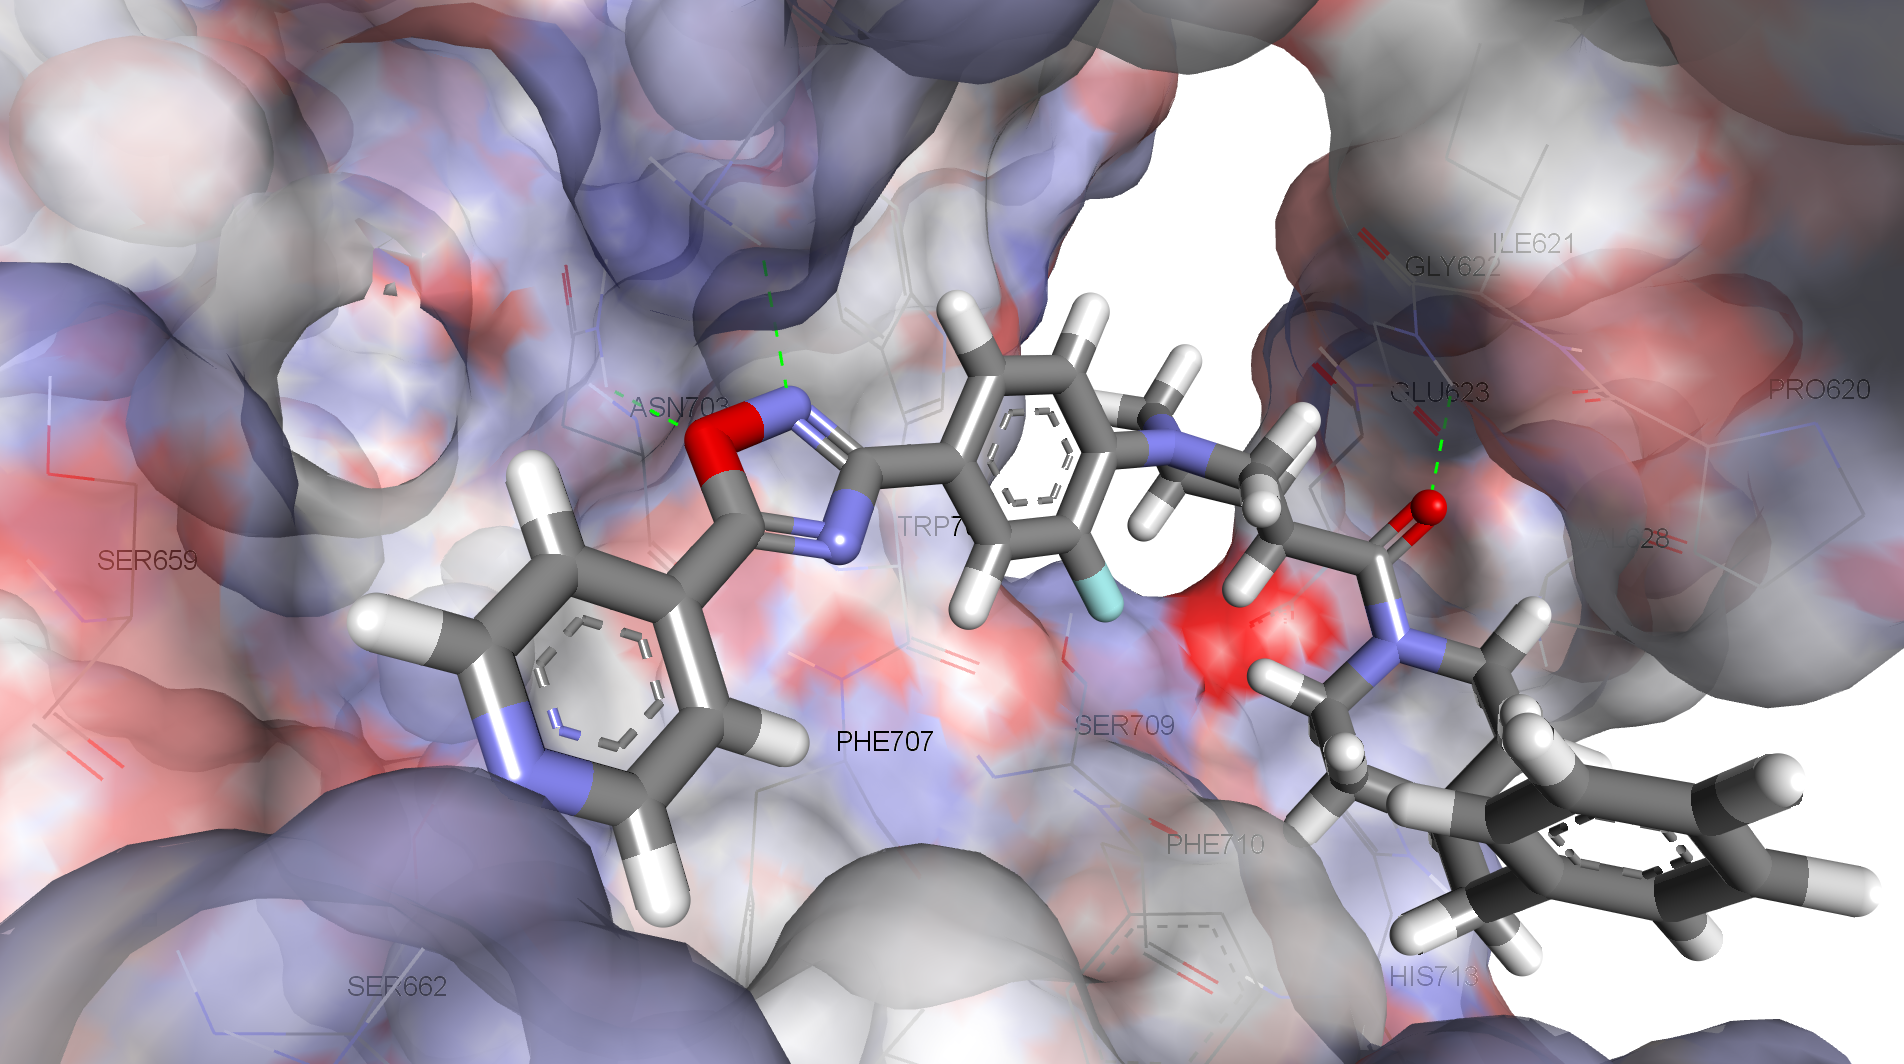
\includegraphics[width=\linewidth]{../influenza/2ZNL-ZINC40879809.png}
\caption{Influenza A RNA polymerase subunit PA in complex of ZINC40879809, which forms 3 hydrogen bonds with GLY622, LYS643 and ASN703, and Pi-Pi interactions with TRP706. Free energy predicted by idock is -11.465 kcal/mol.}
\label{influenza:2ZNL-ZINC40879809}
\end{figure}

\begin{figure}
\centering
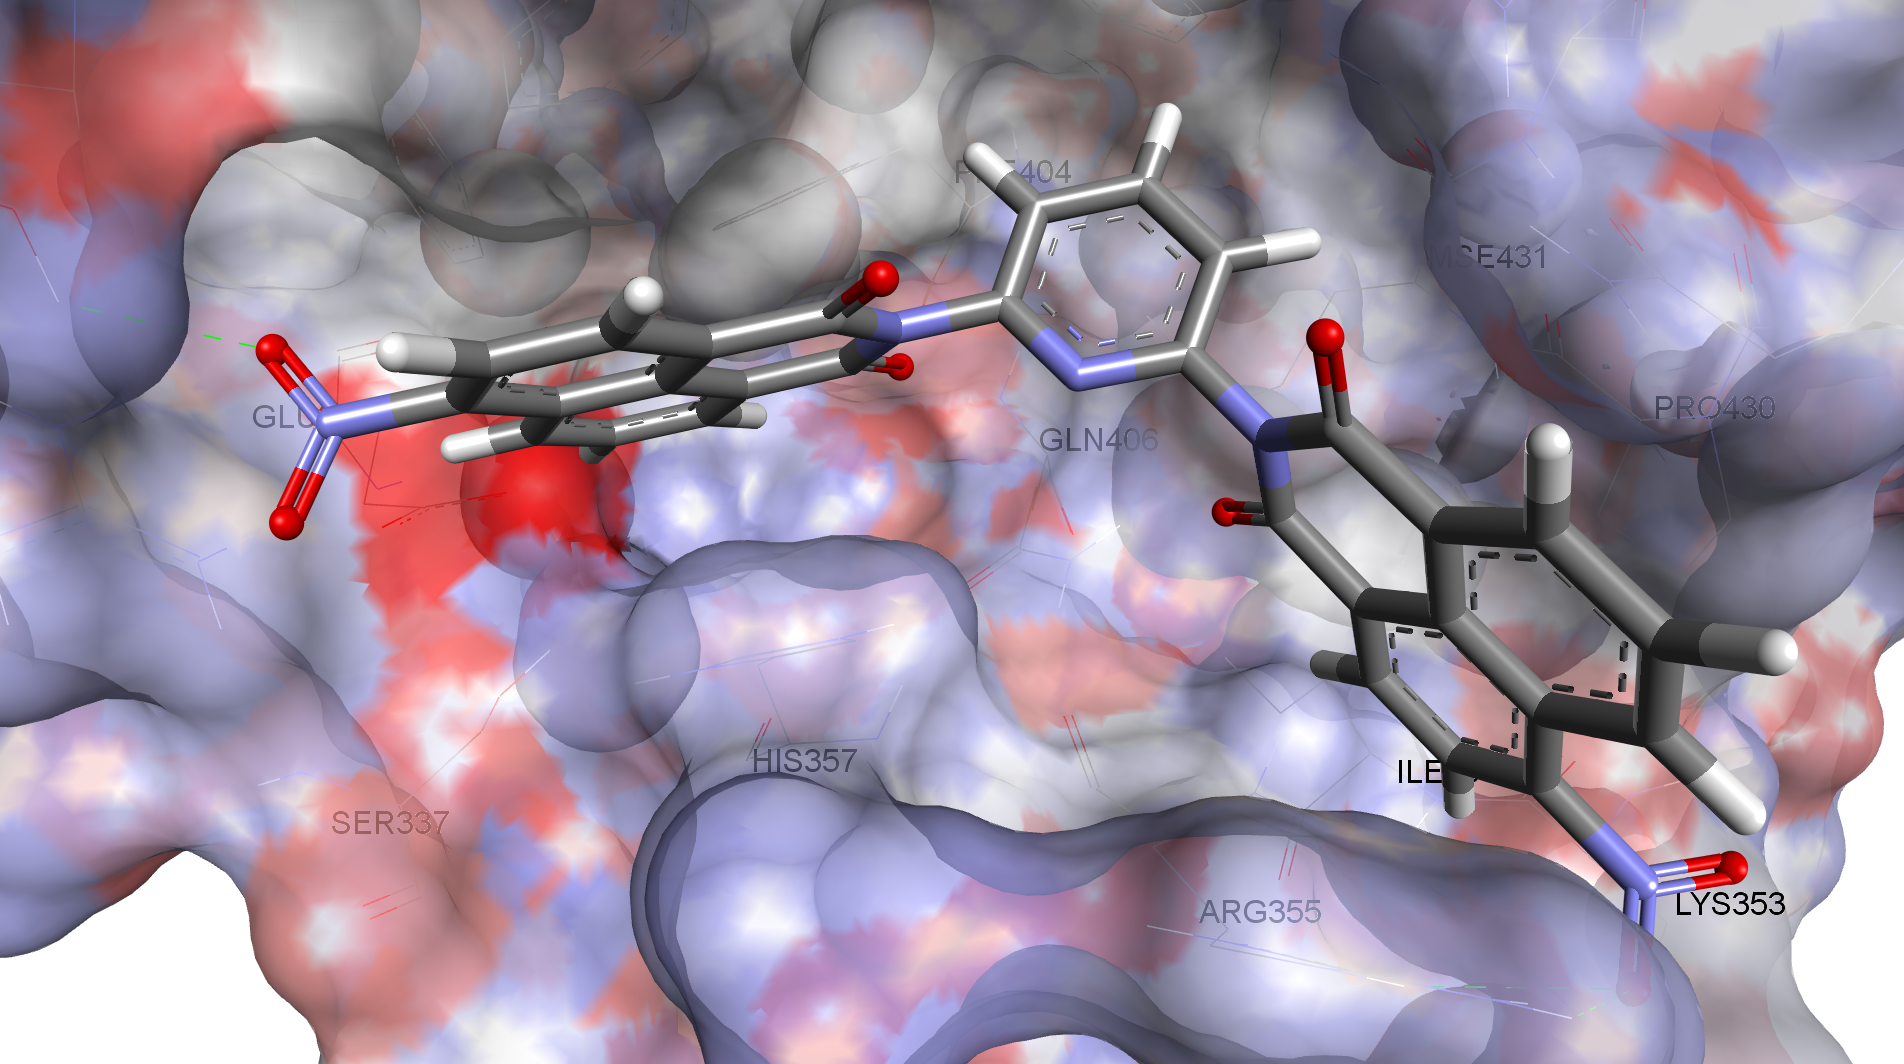
\includegraphics[width=\linewidth]{../influenza/2VQZ-ZINC03015113.png}
\caption{Influenza A RNA polymerase subunit PB2 in complex of ZINC03015113, which forms 3 hydrogen bonds with SER321 and ARG355. Free energy predicted by idock is -11.866 kcal/mol.}
\label{influenza:2VQZ-ZINC03015113}
\end{figure}

\begin{figure}
\centering
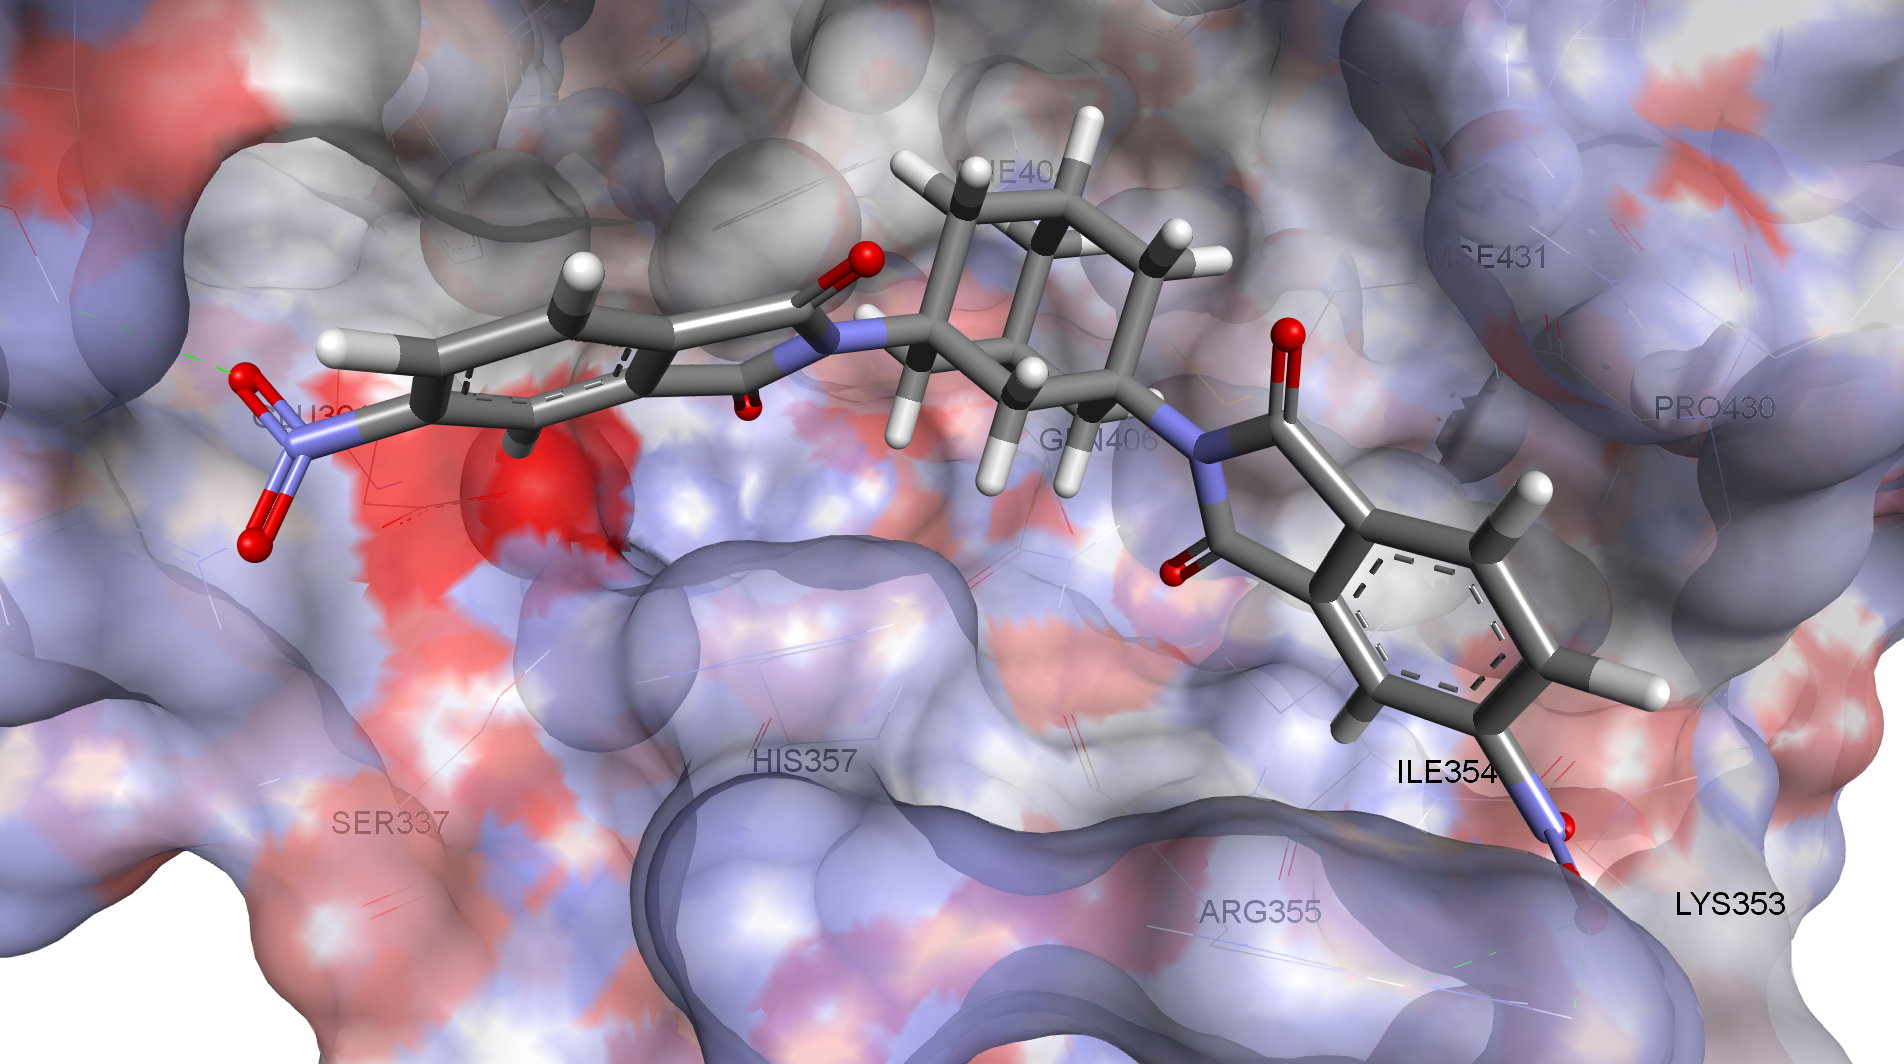
\includegraphics[width=\linewidth]{../influenza/2VQZ-ZINC08386295.png}
\caption{Influenza A RNA polymerase subunit PB2 in complex of ZINC08386295, which forms 3 hydrogen bonds with SER321 and ARG355. Free energy predicted by idock is -12.165 kcal/mol.}
\label{influenza:2VQZ-ZINC08386295}
\end{figure}

\section{Future works}

The top scoring compounds will be subjected to post-screening evaluations, including Lipinski's rule filter, visual inspection and consensus docking using DOCK \citep{1222}, AutoDock Vina \citep{595}, or PLANTS \citep{610,607,779}. The commercially available compounds will be purchased for subsequent biological evaluations.

The cytotoxicity of the compounds will first be tested by MTT assay. Influenza RNP (ribonucleoprotein) reconstitution assay will then be performed to investigate their ability to inhibit RNP transcriptional activity. Hit compounds causing significant reduction of RNP activity will be subjected to whole virus assay including plaque reduction assay and yield reduction assay using seasonal flu viruses. Surface plasmon resonance will also be performed to test the \textit{in vitro} binding affinity of the compounds to the target protein. 

For compounds that exhibit substantial anti-influenza properties, chemical analogues will be purchased for further evaluation. Structure activity relationship study will be performed to further characterize the interaction between the compound and the target protein.

Pure computational studies of prospective virtual screening for a target protein of interest, such as the methyltransferase of the dengue virus \citep{1435}, can be accepted for publication in some journals.

\chapterend
